\documentclass[12pt]{article}
\usepackage{pythonhighlight}
\usepackage{graphicx}
\title{My Karpled Sduff for ze ropodica armz brochect}
\author{Reuben Stick \\ \texttt{Email : Reuben@5t1x.Tech} \\ \texttt{Web : 5t1x.Tech} }

\begin{document}
\maketitle

\section{Raw Python}

\subsection{The Torques Applied onto the Wrist Joint}
\pyth{Tr_W = (M_W * 9.81) * L_W}

\subsection{The Torques Applied onto the Elbow Joint}
\pyth{Tr_E = ((M_W * 9.81) * (math.sqrt(L_W^2 + L_E^2 -(((2) * (L_W) * (L_E)) * (math.cos(A_W)))))) + ((M_E * 9.81) * L_E)}

\subsection{The Torques Applied onto the Shoulder Joint}
\pyth{Tr_S = (M_W * 9.81) * (math.sqrt((math.sqrt(L_W^2 + L_E^2 -(((2) * (L_W) * (L_E)) * (math.cos(A_W)))))^2 + L_S^2 -(((2) * ((math.sqrt(L_W^2 + L_E^2 -(((2) * (L_W) * (L_E)) * (math.cos(A_W)))))) * (L_S)) * (math.cos((A_E - (math.acos(((math.sqrt(L_W^2 + L_E^2 -(((2) * (L_W) * (L_E)) * (math.cos(A_W)))))^2 + L_E^2 - L_W^2)/((2)((math.sqrt(L_W^2 + L_E^2 -(((2) * (L_W) * (L_E)) * (math.cos(A_W))))))(L_E)))))))))) + ((M_E * 9.81) * (math.sqrt(L_E^2 + L_S^2 -(((2) * (L_E) * (L_S)) * (math.cos(A_E)))))) + ((M_S * 9.81) * L_S)}

\section{Formulae}

\subsection{The Torques Applied onto the Wrist Joint}
\begin{equation}
Tr_W = (9.81 \times M_W) \times L_W
\end{equation}


\subsection{The Torques Applied onto the Elbow Joint}
\begin{equation}
Tr_E = ((9.81 \times M_W) \times \sqrt{{L_W}^2 + {L_E}^2-(2\times{L_W}\times{L_E} \times \cos({A_W}))})+ (9.81\times {M_E}\times{L_E})
\end{equation}

\subsection{The Torques Applied onto the Shoulder Joint}
\begin{equation}
Tr_S = ((9.81 \times {M_W}) \times {R_{WS}}) + ((9.81 \times M_E)\times R_{WE})+((9.81 \times M_S)\times R_S)
\end{equation}

\begin{equation}
R_{WS}=\sqrt{{R_{WE}}^2+{L_S}^2-(2 \times {R_{WE}} \times {L_S} \times \cos(A_{E 2})}
\end{equation}

\begin{equation}
R_{WE}=\sqrt{{L_W}^2+{L_E}^2-(2 \times {L_W} \times {L_E} \times \cos({A_W}))}
\end{equation}

\begin{equation}
A_{E 1}=\arccos(\frac{{R_{WE}}^2+{L_E}^2-{L_W}^2}{{2}\times{R_{WE}}\times{L_E}})
\end{equation}

\begin{equation}
A_{E 2} = {A_E} - {A_{E 1}}
\end{equation}

\subsection{zo zad}
yez Im zorry, no I didn't chust vrite this, I Hacdually coted/brogrammed it in LaTeX

\section{Inverse Kinematics for Robotic Arm}

\subsection{Inverse Kinematics Modelling in Octave}
Lengths: \\
\centerline{$L1 = 10 $  Length Of First Arm}
\centerline{$L2 = 7 $  Length of Second arm}
\centerline{$L3 = 4 $  Length of Third arm}
\\[1\baselineskip]
All possible $\theta$ values: \\
\centerline{$\theta 1 = 0:0.1:\pi$  all possible theta1 values}
\centerline{$\theta 2 = 0:0.1:1.5*\pi$  all possible theta2 values}
\centerline{$\theta 3 = 0:0.1:\pi/2$  all possible theta3 values}
\\[1\baselineskip]
Meshgrid: \\
\centerline{$[ \theta{1} $, $ \theta{2} $, $ \theta{3} ] = $ meshgrid} \centerline{$ (\theta1 $,$ \theta2 $, $ \theta3) $  generate grid of angle values}
\\[1\baselineskip]
Compute Coordinates:\\
\centerline{$X = l1 * cos(\theta 1) + l2 * cos(\theta 1 + \theta 2) + l3 * cos(\theta 1 + \theta 2 + \theta 3) $  compute $x$ coordinates}
\centerline{$Y = l1 * sin(\theta 1) + l2 * sin(\theta 1 + \theta 2) + l3 * sin(\theta 1 + \theta 2 + \theta 3) $  compute $y$ coordinates}
\\[1\baselineskip]
Create datasets:\\
\centerline{data $1 = [X(:) Y(:) \theta 1(:)] $ create $x$-$y$-$\theta1$  dataset}
\centerline{data $2 = [X(:) Y(:) \theta 2(:)] $ create $x$-$y$-$\theta2$  dataset}
\centerline{data $3 = [X(:) Y(:) \theta 3(:)] $ create $x$-$y$-$\theta3$  dataset}
\\[1\baselineskip]
Plot:\\
\centerline{plot$(X(:),Y(:),'r.')$}

\begin{figure}
\caption{$X - Y$ coordinates for all $\theta 1$, $\theta 2$, and $\theta 3$ combinations}
\centering
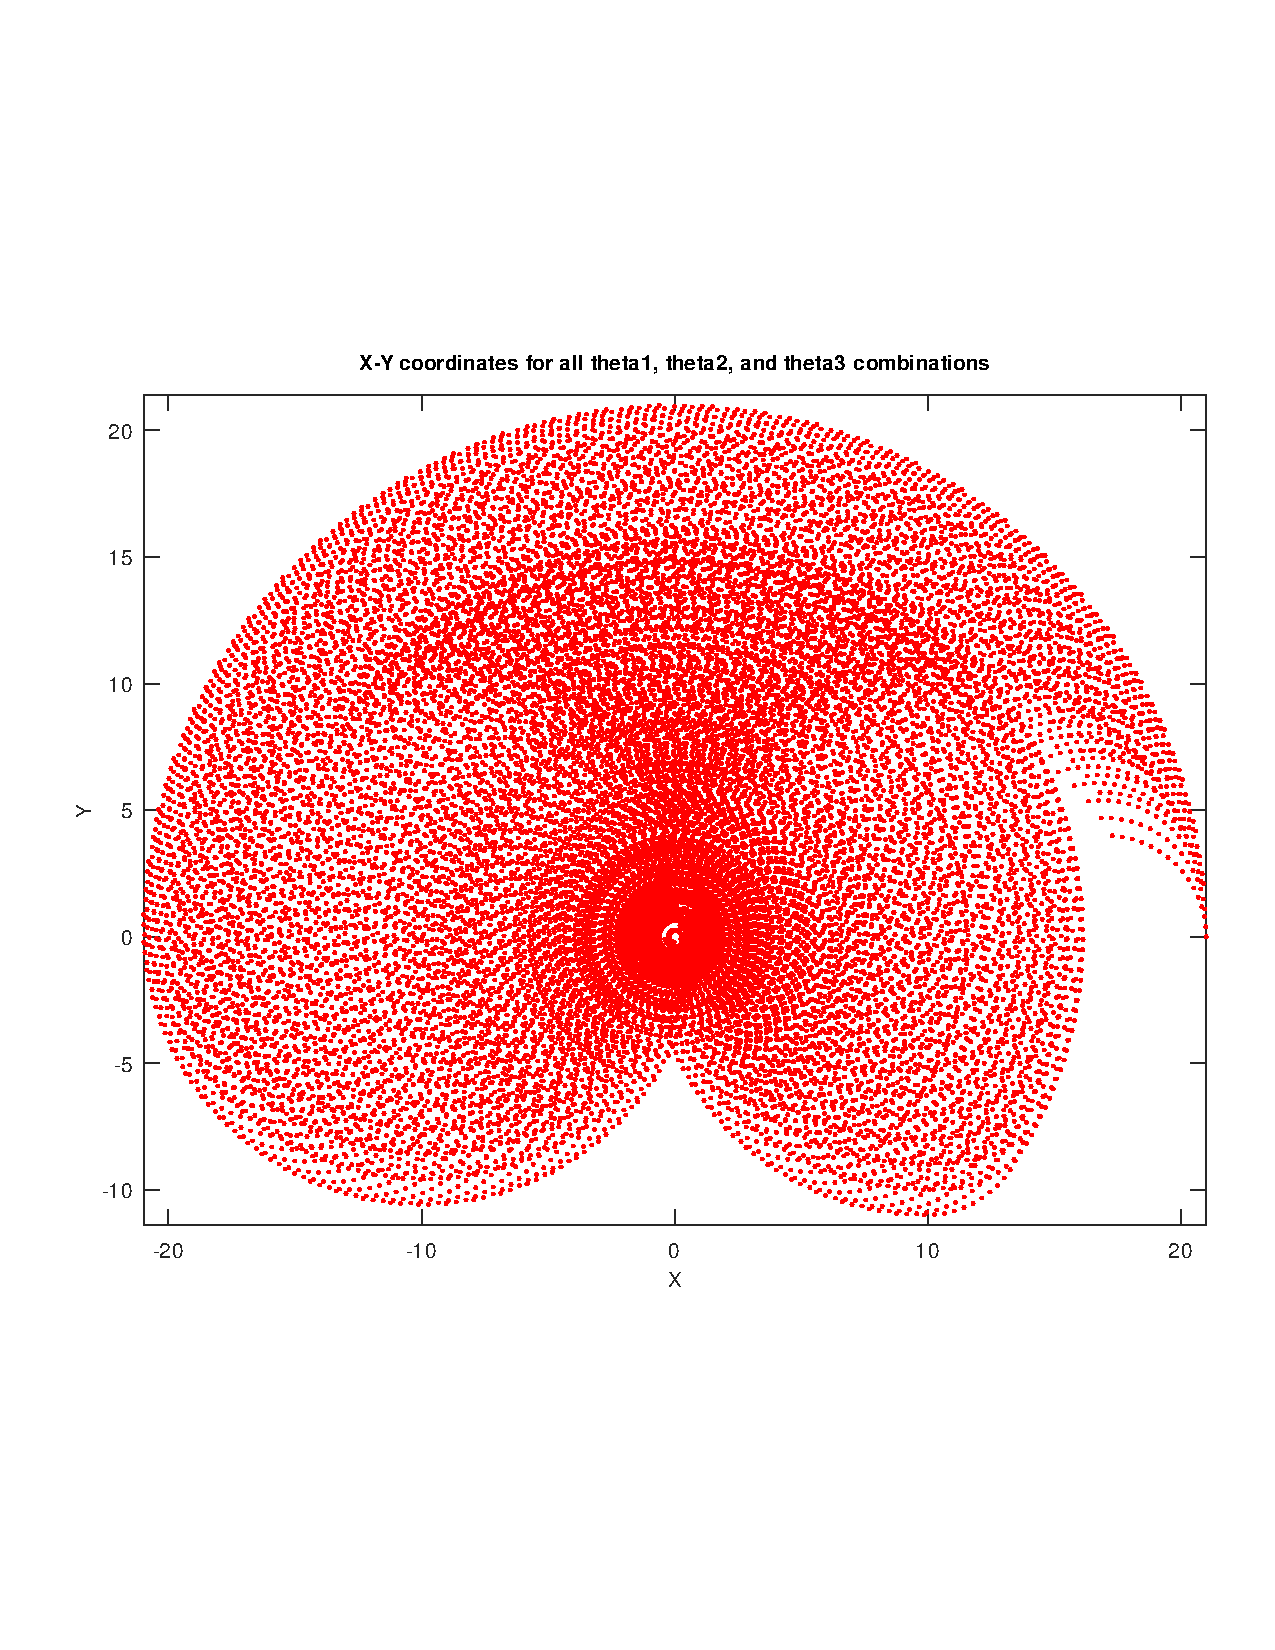
\includegraphics[width=\textwidth]{Inverse Kinematics.pdf} 
\end{figure}

 
\end{document}